% !TEX root = ../main.tex
\chapter{Implementation Details}
%\section{Detailed Validation Results}
\label{chapter:DetailedDescriptions}\label{appendix}
%\inputminted{c++}{../../src/wos_native.cuh}

\chapter{Meta World}
\label{chapter:MetaWorld}

\chapter{Additional Plots}
\label{chapter:additional_plots}

\begin{figure}[htbp]
    \centering
    \begin{subfigure}[b]{0.45\textwidth}
      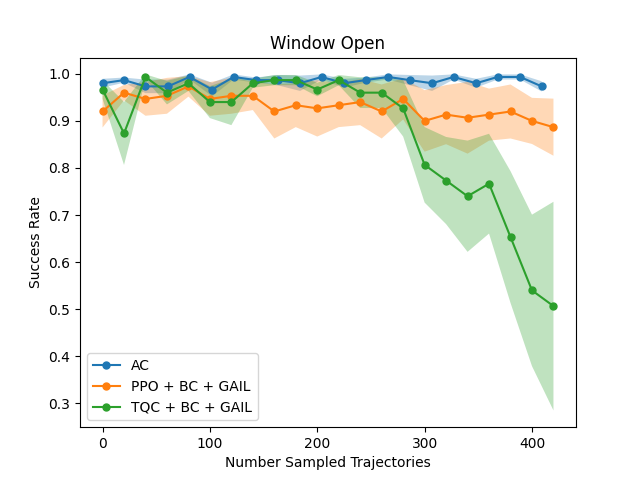
\includegraphics[width=\textwidth]{images/15_400/Window Open.png}
      \caption{Window Open environment.}
      \label{fig:plot1}
    \end{subfigure}
    \hfill
    \begin{subfigure}[b]{0.45\textwidth}
      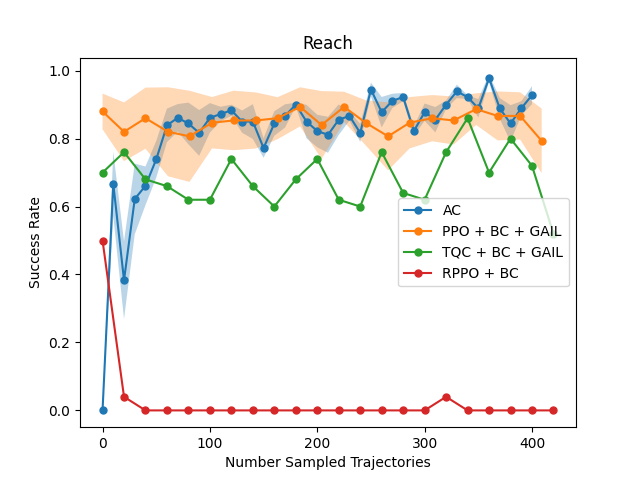
\includegraphics[width=\textwidth]{images/15_400/Reach.png}
      \caption{Reach environment.}
      \label{fig:plot2}
    \end{subfigure}
    \medskip
    \begin{subfigure}[b]{0.45\textwidth}
      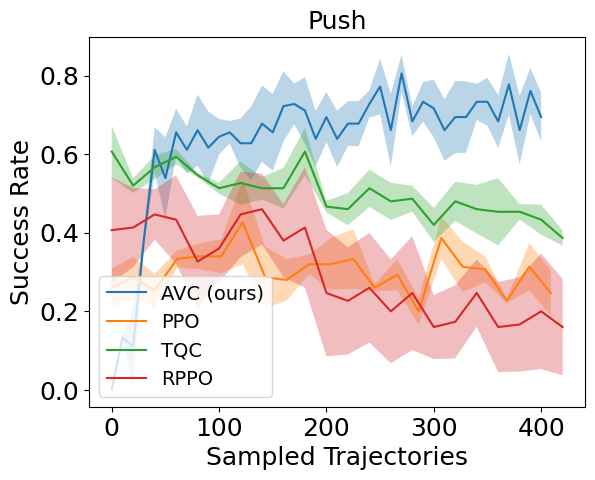
\includegraphics[width=\textwidth]{images/15_400/Push.png}
      \caption{Push environment.}
      \label{fig:plot3}
    \end{subfigure}
    \hfill
    \begin{subfigure}[b]{0.45\textwidth}
      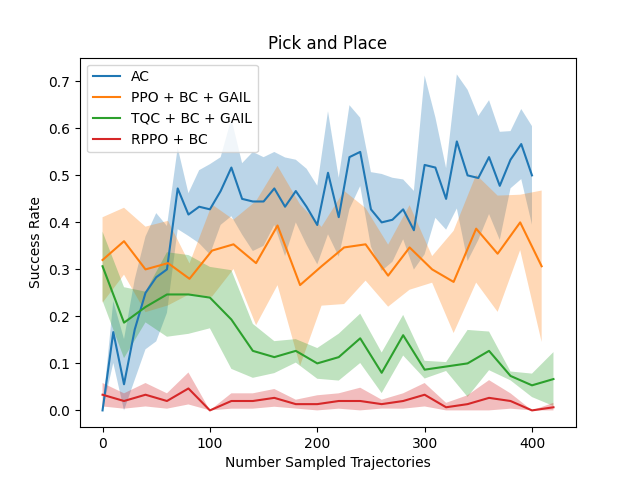
\includegraphics[width=\textwidth]{images/15_400/Pick and Place.png}
      \caption{Pick and Place environment.}
      \label{fig:plot4}
    \end{subfigure}
    \caption{All learners were pretrained using behavioural cloning with the given 15 expert demonstrations. 
    The x-axis shows the number of sampled environment episodes, each with 100 steps.  One initial observation and a sparse reward signal at the end of each episode was provided. 
    The shaded area indicates the standard deviations from four runs per experiment.}
    \label{fig:4}
\end{figure}

\begin{figure}[htbp]
  \centering
  \begin{subfigure}[b]{0.45\textwidth}
    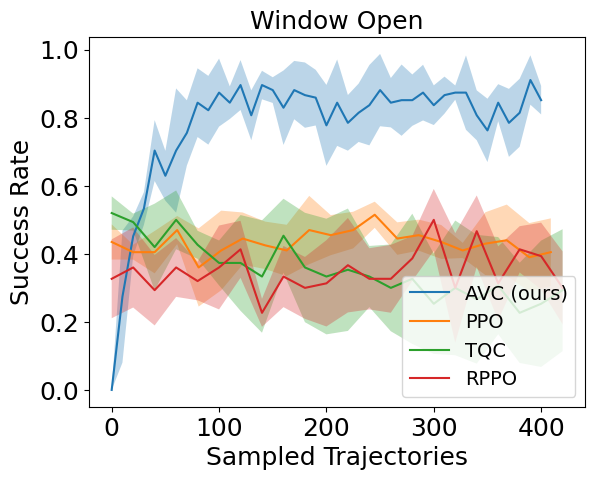
\includegraphics[width=\textwidth]{images/4_400/Window Open.png}
    \caption{Window Open environment.}
    \label{fig:plot1}
  \end{subfigure}
  \hfill
  \begin{subfigure}[b]{0.45\textwidth}
    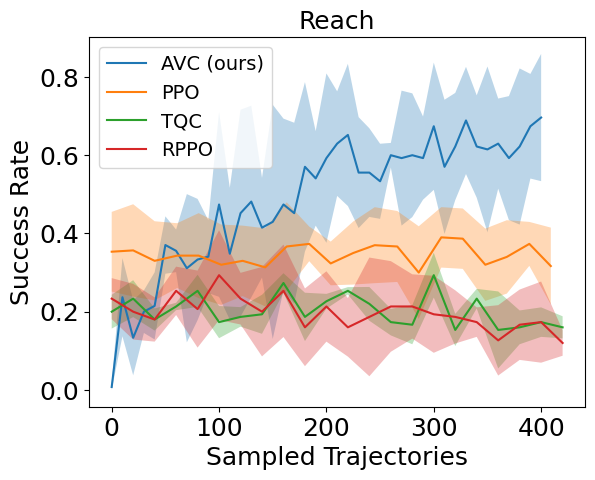
\includegraphics[width=\textwidth]{images/4_400/Reach.png}
    \caption{Reach environment.}
    \label{fig:plot2}
  \end{subfigure}
  \medskip
  \begin{subfigure}[b]{0.45\textwidth}
    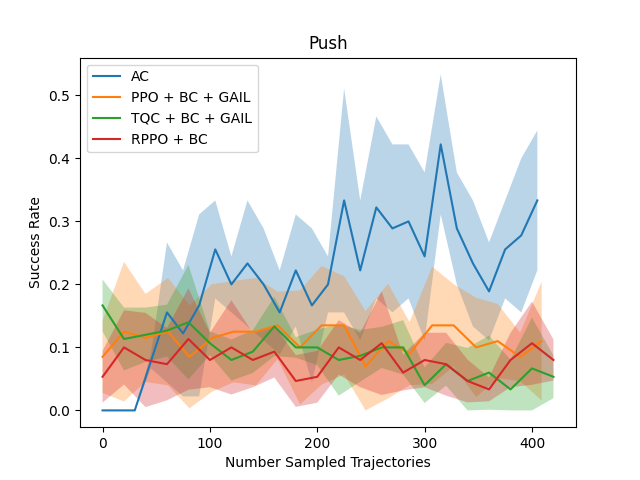
\includegraphics[width=\textwidth]{images/4_400/Push.png}
    \caption{Push environment.}
    \label{fig:plot3}
  \end{subfigure}
  \hfill
  \begin{subfigure}[b]{0.45\textwidth}
    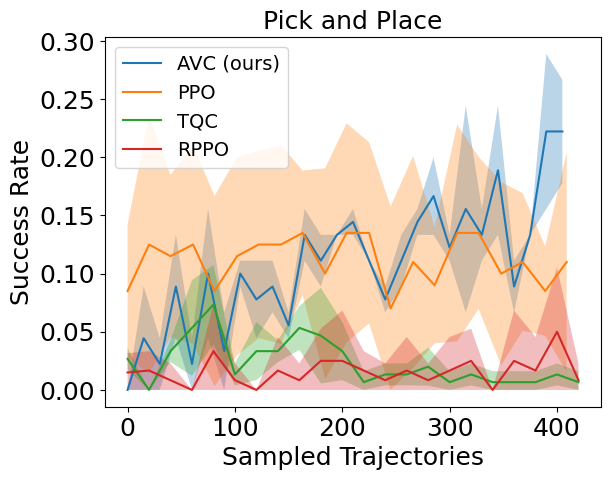
\includegraphics[width=\textwidth]{images/4_400/Pick and Place.png}
    \caption{Pick and Place environment.}
    \label{fig:plot4}
  \end{subfigure}
  \caption{All learners were pretrained using behavioural cloning with the given 4 expert demonstrations. 
  The x-axis shows the number of sampled environment episodes, each with 100 steps.  One initial observation and a sparse reward signal at the end of each episode was provided. 
  The shaded area indicates the standard deviations from four runs per experiment.}
  \label{fig:4}
\end{figure}

\chapter{Generative Adversarial Imitation Learning}
\label{app:GAIL}
For imitation learning, Generative Adversarial Imitation Learning (GAIL) 
\cite{ho2016generative} presents a key paradigm to make efficient use of expert demonstrations given access to the MDP. 
The main idea of GAIL is to disambiguate the reward signal 
by ensuring every policy except the expert policy has a lower expected reward under our inverse reward function, given the expert 
demonstrations.\\ 
First, 
maximum causal entropy IRL \cite{10.5555/3104322.3104481} is a method to regularize policies found from inverse reinforcement learning. The idea is to choose the reward function, for 
which the optimal policy has the highest entropy with respect to the action distribution. This allows us to choose a policy that is "no more committed to any 
particular path" \cite[p.2]{10.5555/3104322.3104481}, then necessary. Formally the objective is written as:
\begin{equation*}
    \label{proto_inf_ler}
    \underset{r_{\text{inv}} \in \mathcal{R}}{\text{minimize}} \left( \max_{\pi \in \Pi} \left( - \text{H}(\pi) + \mathbb{E}_{\pi}[r_{\text{inv}}(s, a)] \right) - \mathbb{E}_{\pi_{r'}^*}[r_{\text{inv}}(s,a)] \right),
\end{equation*}
with the discounted expected reward
\begin{equation*}
    \mathbb{E}_{\pi}[r(s, a)] =
    \mathbb{E}_{(s,a,t) \propto \pi}[\gamma^t r(s,a)] = 
    \mathbb{E}_{\tau \sim p(\tau | \pi)} \left[ \sum_{t=0}^\infty \gamma^t r_t \right]
\end{equation*}
and the discounted causal entropy as defined by Bloem, et al. \cite{InfCausalEnt}:
\begin{equation*}
    \mathbb{H}(\pi) = \mathbb{E}_{s_0, a_0} \left(\text{H}_{\pi}(a_{0...\infty}, s_{0,...\infty})\right) = \mathbb{E}_{\pi}\left[\sum_{t=0}^\infty -\gamma^t log \pi(a_t|s_t)\right].
\end{equation*}
Here $\pi_{r'}^*$ denotes the expert policy, which indicates the expert policy is assumed to maximise a true 
reward function ${r'}$. From now, we will refer to the expert policy as $\pi_{\text{E}}$, as it is more in line with the common choice found in 
literature. Furthermore, we used the reward in equation  \ref{proto_inf_ler}, as it is in line with our notation for reinforcement learning. In the paper, 
the authors minimize a cost function $c$, instead of maximzing a reward function $r$. The choice does not make a profound 
mathematical difference, but it gives a more natural way to interpret the inverse objective. $c=0$ can be naturally defined as the optimal cost value, while a reward function has 
no natural upper bound. For this practical reason, we will make use of $c$ instead of $r$ for the rest of this section. As $c \propto -r$, the minimisation in 
\ref{proto_inf_ler} becomes a maximization and vice versa:
\begin{equation}
    \label{proto_inf_ler_c}
    \pi_{\text{inv}}^* = \underset{c_{\text{inv}} \in \mathcal{C}}{\text{max}} \left( \min_{\pi \in \Pi} \left(- \text{H}(\pi) + \mathbb{E}_{\pi}[c_{\text{inv}}(s, a)] \right) - \mathbb{E}_{\pi_{\text{E}}}[c_{\text{inv}}(s,a)] \right).
\end{equation}
The key insight is, that this optimisation problem can be uniquely identified with an occupancy measure distance between the expert policy and the 
induced policy. Intuitively, an occupancy measure is a measure for how likely a policy visits a state action pair given the MDP. If two policies visit the same 
states and choose the same actions, they are similar to each other.\\
Formally the occupancy measure for states and actions is defined by: 
\begin{equation*}
    \rho_{\pi}:\mathcal{S} \times \mathcal{A} \rightarrow \mathbb{R} = \pi(a|s)\sum_{t=0}^\infty \gamma^tP(s_t=s|\pi).
\end{equation*}
With this, the discounted expected reward can be written as:
\begin{equation}
    \mathbb{E}_\pi[c(s,a)] = \sum_{s,a} \rho_\pi(s,a) c(s,a)
\end{equation}
and equation \ref{proto_inf_ler_c} can be written as:
\begin{equation}
    \label{occ_meas_obj}
    \pi_{\text{inv}}^* = \max_{c_{\text{inv}} \in \mathcal{C}} \left( \min_{\rho_\pi \propto \pi \in \Pi} \left(- \bar{\text{H}}(\rho_\pi) + \sum_{s,a} \rho_\pi(s,a) c(s,a) \right) - \sum_{s,a} \rho_{\text{E}}(s,a) c(s,a) \right).
\end{equation}

It is then shown that a policy is uniquely identified with its occupancy measure $\rho_{\pi} \propto \pi$. With this in mind, we rewrite equation \ref{proto_inf_ler_c} as a constrained satisfaction problem:
\begin{equation}
    \label{const_sat_gail}
    \pi_{\text{inv}}^* = \min_{\pi \propto \rho_{\pi}} - \bar{\text{H}}(\rho_{\pi})\quad \text{subject to }\quad \rho_{\pi}(s,a) = \rho_{\text{E}}(s,a) \quad \forall s \in \mathcal{S}, \forall a \in \mathcal{A},
\end{equation}
where $\bar{\text{H}}$ is the the discounted causal entropy $\text{H}$ defined on occupancy measures of policies, rather then action distributions. In this sense, equation \ref{proto_inf_ler_c} is the dual problem of equation \ref{const_sat_gail}. 
This optimisation is intractable, as we get as many constraints, as we have action state pairs in our MDP. Moreover, in practice we only have a small sample size, which would mean setting 
the occupancy measure for all unvisited state action pairs to zero. This is obviously not the intended optimum. Instead, the objective \ref{const_sat_gail} is relaxed:
\begin{equation}
    \label{dist_opt}
    \pi_{\text{inv}}^* = \min_{\pi} d_{\psi}(\rho_{\pi_{\text{E}}}, \rho_{\pi}) - \text{H}(\pi)
\end{equation}
such that $d_{\psi}$ becomes small, when $\pi_{\text{E}}$ and $\rho_{\pi}$ become similar. To do this, we can introduce an additional regularizor $\psi$ to equation \ref{occ_meas_obj}:

\begin{equation*}
    \pi_{\text{inv}}^* = \max_{c_{\text{inv}} \in \mathcal{C}} \left(-\psi(c) \ \min_{\rho_\pi \propto \pi \in \Pi} \left(- \bar{\text{H}}(\rho_\pi) + \sum_{s,a} \rho_\pi(s,a) c(s,a) \right) - \sum_{s,a} \rho_{\text{E}}(s,a) c(s,a) \right)
\end{equation*}
\begin{equation*}
    = \min_{\rho_\pi \propto \pi \in \Pi}- \bar{\text{H}}(\rho_\pi) + \max_{c_{\text{inv}} + \in \mathcal{C}} -\psi(c) \sum_{s,a} \left( \rho_\pi(s,a) - \rho_{\text{E}}(s,a)\right) c(s,a)
\end{equation*}
\begin{equation}
    \label{proto_inf_ler_c_reg}
    = \min_{\rho_\pi \propto \pi \in \Pi}- \bar{\text{H}}(\rho_\pi) + \psi^*(\rho_\pi(s,a) - \rho_{\text{E}}(s,a)),
\end{equation}
where $\psi^*$ is the complex conjugate of $\psi$. With this, we can identify $d_{\psi} = \psi^*$.\\

What is left now is to find a $\psi$ s.t. minimizing \ref{dist_opt} ensures $\rho_{\pi} \sim \rho_{\test{E}}$. The authors propose $\psi_{\text{GA}}$, 
which complex conjugate $\psi^*_{\text{GA}}$ is: 
\begin{equation}
    \psi^*_{\text{GA}} = \max_{D\in(0,1)^{\mathcal{S} \times \mathcal{A}}} \mathbb{E}_{\pi}\left[ \text{log}(D(s,a))\right] + \mathbb{E}_{\pi_{\text{E}}}\left[ \text{log}(1 - D(s,a))\right],
\end{equation}
with discriminator $D$. In this formulation, the objective \ref{proto_inf_ler_c_reg} minimzes the Jensen Shannon divergence ($D_{JS}$) between $\rho_\pi$ and $\rho_{\text{E}}$. If we treat the entropy constraint as a regularisation with 
parameter $\lambda$, the GAIL objective can be written as:
\begin{equation}
    J(\rho_{\pi_{\theta}}, D_{\omega}) = - \lambda  \bar{\text{H}}(\rho_{\pi_{\theta}} ) + \mathbb{E}_{\pi_{\theta}}\left[ \text{log}(D_{\omega}(s,a))\right] + \mathbb{E}_{\pi_{\text{E}}}\left[ \text{log}(1 - D_{\omega}(s,a))\right],
\end{equation}
where $\omega$ and $\theta$ denote the parametrization of the discriminator $D$ and the policy $\pi$. Identifying the discounted reward as $Q = \mathbb{E}_{\pi}(r_t) = \mathbb{E}_{\pi}\left[-\text{log}(D_{\omega}(s,a))\right]$ and unsing the policy 
gradient theorem, we get the policy update rule:
\begin{equation}
    \label{GAIL_update_policy}
    \nabla_{\theta} J(\rho_{\pi_{\theta}}, D_{\omega}) = \mathbb{E}_{\tau \propto \pi}\left[ \nabla_{\theta}\text{log}\pi_{\theta}(a|s) Q(s,a) -\lambda \nabla_{\theta}\bar{\text{H}}(\rho_{\pi_{\theta}} )  \right]
\end{equation}
and the discrimnator update rule as:
\begin{equation}
    \label{eq_GAIL_disc}
    \nabla_{\omega} J(\rho_{\pi_{\theta}}, D_{\omega}) = \mathbb{E}_{\tau \propto \pi} [\nabla_w \log(D_w(s,a))] + {E}_{\tau_E} [\nabla_w \log(1 - D_w(s,a))].
\end{equation}
Note, because cost $c$ instead of reward $r$ is used in equation \ref{GAIL_update_policy} gradient descent is used, as the cost is minimized and in equation \ref{eq_GAIL_disc} 
gradient ascent is used, as we want to maximise the discriminative power of $D$. The algorithm is summarized in algorithm \ref{GAIL_Algo}.\\ \\
\begin{algorithm}
    \caption{Generative adversarial imitation learning}
    \label{GAIL_Algo}
    \begin{algorithmic}
    \Require Expert trajectories $\tau_E \sim \pi_E$, initial policy and discriminator parameters $\theta_0$, $w_0$\\
    \For{$i = 0, 1, 2, \dots$}{\\
        \State Sample trajectories $\tau_i \sim \pi_{\theta_i}$\\
        \State Update the discriminator parameters from $w_i$ to $w_{i+1}$ with the gradient\\
            \begin{equation}
            \hat{\mathbb{E}}_{\tau_i} [\nabla_w \log D_w(s, a)] + \hat{\mathbb{E}}_{\tau_E} [\nabla_w \log(1 - D_w(s, a))]
            \end{equation}
        \State Take a policy step from $\theta_i$ to $\theta_{i+1}$, using the TRPO rule with cost function $\log D_{w_{i+1}}(s, a)$.\\
        Specifically, take a KL-constrained natural gradient step with\\
        \begin{equation}
        \hat{\mathbb{E}}_{\tau_i} [\nabla\theta \log \pi_\theta(a|s)Q(s, a)] - \lambda \nabla_\theta H(\pi_\theta),
        \end{equation}
        where $Q(\bar{s}, \bar{a}) = \hat{\mathbb{E}}_{\tau_i} [\log D{w_{i+1}}(s, a) | s_0 = \bar{s}, a_0 = \bar{a}]$\\
    \EndFor}
    \end{algorithmic}
    \end{algorithm}
Tian Xu, et al. proved that if a policy $\pi$ minimizes the $\text{D}_{JS}$ distance 
between occupancy measures of $\rho_{\pi^*}$ and $\rho_{\pi}$, the generalization error $V_{\pi^*} - V_{\pi_{\text{imitation}}}$ is bound by 
$V^{{\pi^*}} - V^{\pi} \leq \mathcal{O}\left(\frac{1}{\sqrt{1-\gamma}}\right)$, while the generalization error of behavioural cloning is bound by 
$V^{{\pi^*}} - V^{\pi} \leq \mathcal{O}\left(\frac{1}{\sqrt{1-\gamma^2}}\right)$ \cite{NEURIPS2020_b5c01503} . This explains better performance for GAIL in long horizon tasks, which has 
been empirically demonstrated. Overall, GAIL is a state-of-the-art imitation learning algorithm which is able to learn complex behaviour with limited expert demonstrations. It shows outstanding 
asymptotical performance with respect to the amount of expert demonstrations but requires a high number of enviroment interactions to train the discriminator and actor as stated by the authors. 

\chapter{Language-Conditioned Imitation Learning for Robot Manipulation Tasks}
\label{LCILRM}
Simon Stepputtis et al. \cite{stepputtis2020languageconditioned} propose a benchmark for natural language conditioned robot manipulation tasks. \\
The benchmark consists of a 7 dof simulated robot arm with a 
tabletop setup using CoppeliaSim, which allows for accurate dynamics simulations at an update rate of 20 Hz. 
An imitation learning dataset consisting of 44 100 tasks is provieded, where 4000 tasks are used for 
evaluation and 100 tasks are used for testing.\\

The task consists of picking up objects and pouring their content into other objects. A sentense in natural language describes the task and the object. 
For example "Pick up the red cup". Additionally, an rgb image of the scene is provided. An overview over 
all possible objects and an example task can be found in figure \ref{lang_imi_expl}. 
There is only one observation per trajectory, so the setting is the single observation POMDP.  \\


Simon Stepputtis et al. \cite{stepputtis2020languageconditioned} also propose a method to solve the benchmark. 
The proposed method involves using a neural network to map natural language instructions to 
corresponding robot actions. The experimental results demonstrate the effectiveness of their approach in inferring and executing trajectories for robot manipulation 
tasks when language instructions are given. \\

In more detail, a policy $\pi(v,I)$ is learned to imitate expert behaviour in a set of demonstrations $D = \{d_0,...,d_m\}$, each containing a trajectory 
$R \in R^{T \times N}$ over $T$ time steps and with $N$ control variables, an rgb image $I \in \mathcal{R}^{569 \times 320 \times 3}$ of the agent's surroundings, 
and a task description $v \in \mathcal{R}^{15 \times 50}$ from natural language. The proposed method takes the image $I$ and task description $v$ 
to create a task embedding $e$ using GloVe embeddings and a pretrained image recognition model in the semantic model, 
which is subsequently used in the control model to generate robot actions at each timestep in a closed-loop 
fashion using a GRU to keep track of the former history. In addition to the hidden state of the GRU, 
the task embedding $e$ is used in every timestep, as we know, that the task does not change. A schematic overview can be seen in figure \ref{language_imitation}. \\

\begin{figure}[htbp]
    \centering
    \includegraphics[width=\textwidth]{images/Language_Conditioned/System.pdf}
    \caption{Overview of the general system architecture. (Left) Details of the controller model, which
    synthesises robot control signals . (Right) details of the semantic model, which extracts critical
    information about the task from both perceptual input and language commands. Dark-blue boxes
    indicate pre-trained components of the model. The figure is taken from \cite{stepputtis2020languageconditioned}.}
    \label{language_imitation}
\end{figure}

The authors find that their model can perform $98 \%$ of pick tasks, $85 \%$ of pour tasks and $84 \%$ combined 
tasks, which greatly outperforms a baseline using an end to end RNN model with $58\%$ success rate for picking and $0 \%$ success rate for pouring.

\begin{figure}[htbp]
    \centering
    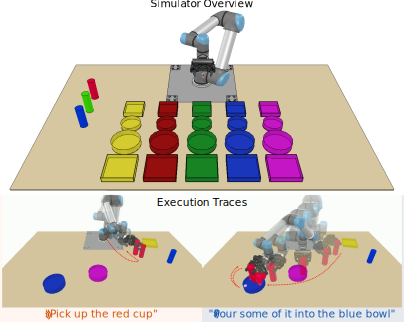
\includegraphics[width=0.4\textwidth]{images/Language_Conditioned/simulator.pdf}
    \caption{Overview of a task. (top) All possible objects and colors. (left) Example trajectory to "pick up the red cup" following the natural language description. 
    (right) Example trajectory to "pour some of it into the blue bowl". The figure is taken from \cite{stepputtis2020languageconditioned}.}
    \label{lang_imi_expl}
\end{figure}
